\documentclass[letter,11pt]{article}
\usepackage{animate}
\usepackage{listings}
\usepackage{color}
\usepackage[utf8]{inputenc}
\usepackage[math,]{kurier}
\usepackage[T1]{fontenc}
\usepackage{microtype}
\usepackage{wrapfig}
\usepackage[columnsep=10pt,left=2cm,top=2.3cm,right=2cm,bottom=2.3cm]{geometry}
\usepackage[hang, small,labelfont=bf,up,textfont=it,up]{caption}\usepackage{booktabs}
\usepackage{lettrine} % The lettrine is the first enlarged
\usepackage{paralist} % Used for the compactitem environment
\usepackage{mathtools}
\usepackage{abstract} % Allows abstract customization
\renewcommand{\abstractnamefont}{\normalfont\bfseries\large} %Set the "Abstract" text to bold
\renewcommand{\abstracttextfont}{\normalfont\small\itshape} %Set the abstract itself to small italic text
\usepackage{graphicx}
\usepackage[spanish,mexico]{babel}
\usepackage{amsmath} %simbolos matematicos
\usepackage{multicol}  %texto a varias columnas
\usepackage{enumerate}
\usepackage{float} 
\usepackage{fancyhdr} % Headers and footers
\pagestyle{fancy} % All pages have headers and footers
\fancyhead[]{} % Blank out the default header
\fancyfoot{} % Blank out the default footer
\fancyhead[L]{} % Custom header text
\fancyfoot[C]{\thepage} % Custom footer text
\usepackage{hyperref}
\hypersetup{
    colorlinks,
    citecolor=black,
    filecolor=black,
    linkcolor=black,
    urlcolor=black
}


\title{Oscilaciones en Sistemas biológicos}
\author{Alejandro Hernández de la Vega \\ César Daniel Rodríguez Rosenblueth \\ Eva Yazmín Santiago Santos}
\date{}

\begin{document}

\maketitle

\tableofcontents

\pagebreak


\section{Osciladores Biológicos}

Bien sea la respiración, la elaboración de marcapasos para asistir la actividad cardiaca o la secreción de testosterona en los hombres, existen varios sistemas biológicos que exhiben un carácter oscilatorio. Una primera aproximación para el estudio de estos sistemas desemboca en ecuaciones diferenciales ordinarias del tipo:

$$\dfrac{du}{dt} = f(u)$$

Donde, para sistemas periódicos se tiene:

$$u(t+T)= (t) $$

con el periodo $T>0$

No obstante, existen casos (como en la síntesis de enzimas durante la división celular o en el estudiado en este trabajo) donde el sistema viene regulado por un control de retroalimentación. En este sentido, el sistema viene dado por una serie de reacciones ligadas, llevándose acabo una reacción seguida de otra y en donde la primera de éstas viene regulada por una función de retroalimentación que involucra la última reacción, i.e. si tenemos n reacciones:
$$ \dfrac{d u_1}{dt} = f(u_n )k_1 u_1 $$ 
$$ \dfrac{d u_r}{dt}= u_{r-1} -k_r u_r $$

con $r=2,3,...,n$ , $ k_r > 0 $ constantes determinadas por el sistema en cuestión y $ f(u)$ la función de retroalimentación.

Los trabajos de Tyson y de Othmer(1978) y Yagil (1971) muestran que la función de retroalimentación tiene que ser una función siempre positiva y monótona decreciente para asegurar la unicidad de las soluciones de estado estacionario.

\section{Características de la Testosterona}

La testosterona es una hormona cuya función principal es estimular el desarrollo de los caracteres sexuales masculinos, y está presente en mamíferos, reptiles y aves. Para el ser humano, en los hombres el nivel de testosterona se encuentra entre 10-35 nanomoles por litro de sangre, mientras que en las mujeres es de 0.7-2.7 nanomoles por litro. La testosterona es principalmente producida en los testículos en los hombres y en los ovarios de las mujeres, en los hombres, los niveles de testoterona oscilan con un periodo de 2 a 3 horas.

Existen cambios de personalidad relacionados con la concentración de testosterona en la sangre, por ejemplo niveles bajos de testosterona vienen acompañados con actitudes dóciles en los sujetos, además, pacientes que padecen de cáncer de próstata, son sometidos a un tratamiento que involucra la toma de Goserelina, una droga que al término de un par de semanas reduce el nivel de testosterona al grado que se alcanzaría a través de la castración. 

\subsection{Secreción de la Testosterona}

La secreción de testosterona (T) por parte de las gónadas viene regulada por la hormona luteinizante (LH) generada en la glándula pituitaria, esta última viene regulada, a su vez, por la hormona liberadora de hormona luteinizante (LHRH) que es secretada en el hipotálamo. Además la testosterona ejerce una retroalimentación en la producción de LHRH. 

Entonces, en este sistema, el hipotálamo secreta hormona liberadora de hormona luteinizante que es llevada a través del torrente sanguíneo a la glándula pituitaria, donde se controla la secreción de hormona luteinizante que finalmente controla la producción de testosterona en las gónadas, es entonces que se ejerce la retroalimentación entre de los testículos hacia el hipotálamo.\\

Se denota a T, LH y LHRH por $T(t) L(t)$ y $R(t)$ respectivamente. Para una primera aproximación se utiliza el siguiente modelo:

\begin{center}
 \includegraphics[width=3in]{imagenes/Diagramas/diagram2.png}
\end{center}

Donde el comportamiento del sistema está representado por las siguientes ecuaciones.

\begin{equation}
\frac{dR}{dt} = f(T)-b_{1}R
\label{eqdr}
\end{equation}

\begin{equation}
\frac{dL}{dt} = g_{1}R-b_{2}L
\label{eqdl}
\end{equation}

\begin{equation}
 \frac{dT}{dt} = g_{2}L-b_{3}T 
 \label{eqdt}
\end{equation}


Matemáticamente $b_{1}$, $b_{2}$, $b_{3}$, $g_{1}$, $g_{2}$ son parámetros positivos. Biológicamente $g_{1}$,$g_{2}$ y $f(T)$ son las tasas de secreción de las hormonas LHRH, LH y T respectivamente. Además  $g_{1}$,$g_{2}$ son los valores de prealimentación para R y L respectivamente, mientras que f(T) es una función de retroalimentación para las dos hormonas precursoras. Por tanto deben estar representadas por funciones monótonas crecientes. Por otro lado $b_{1}$, $b_{2}$, $b_{3}$ represetan la tasa de difusión de las hormonas en el torrent sanguinio. Ambos están dados en valores de concentración por hora.

A este modelo general se le llama "feedback repression model". Para los puntos de estabilidad se tiene lo siguiente:\\

Las ecuaciones \ref{eqdl}, \ref{eqdr} y \ref{eqdt} tienen sólución en

$$R_{0} = \frac{f(T_{0})}{b_{1}}$$

$$L_{0} = \frac{b_{3}}{g_{2}}T_{0}$$

Donde $T_{0}>0$ satisface $g_{1}g_{2}f(T_{0}) = b_{1}b_{2}b_{3}T_{0}.$\\

Cuando $f'(T_{0}) < 0$ no hay estabilidad: 

(i) si y sólo si 

$$-\frac{g_{1}g_{2}f'(T_{0})}{b_{1}} > \frac{a_{1}a_{2}}{a_{3}}-1$$

Donde:

$$a_{1} = b_{1}+b_{2}+b_{3}$$
$$a_{2}=b_{1}b_{2}+b_{1}b_{3}+b_{2}b_{3}$$
$$a_{3}=b_{1}b_{2}b_{3}$$

(ii) si 

$$-\frac{T_{0}f'(T_{0})}{f(T_{0})} > 8 $$\\

Alrededor del punto de equilibrio:

$$ \frac{dx}{dt} = f'(T_{0})z-b_{1}x$$
$$ \frac{dy}{dt} = g_{1}x-b_{2}y $$
$$ \frac{dz}{dt} = g_{2}yt-b_{3}T $$

Donde
$$ z(t)=T(t)-T_{0} $$
$$ y(t)=L(t)-L_{0} $$
$$ x(t)=R(t)-R_{0} $$

\section*{Modelo para la esquizofrenia catatónica}

Danzinger y Elmergreen postularon en (1956) un trabajo (analziado posteriormente por Cronin en 1976) en donde se modela matemáticamente la esquizofrenia catatónica periódica, este modelo es similar a:

$$ \frac{dR}{dt} = f(T)-b_{1}R$$
$$ \frac{dL}{dt} = g_{1}R-b_{2}L $$
$$ \frac{dT}{dt} = g_{2}L-b_{3}T $$

pero la función de retroalimentación f(t) que emplearon en este caso es de la forma:

$$ f(z) = (c-hz)[1-H(z-c/h)]  $$

Donde $H(z)$ es la función escalón de Heaviside y $c,h$ son constantes y en donde los criterios de inestabilidad son (7) son:

$$ K = \dfrac{g_1 g_2 h}{b_1 b_2 b_3} > \dfrac{a_1 a_2}{a_3} - 1 $$

Dejando el criterio para (9):

$$ K = \dfrac{g_1 g_2 h}{b_1 b_2 b_3} > 8 $$ 

El análisis de Cronin mostró que cuando el punto de equilibrio es estable, no existen soluciones periódicas, sin embargo, cuando el punto de equilibrio es inestable las soluciones son periódicas, casi periódicas u oscilan de manera no peródica.

Desde el punto de vista fisiológico, el modelo descrito por Danzinger y Elmergreen remplaza R, L, T por la hormona tirotropina, una enzima intermediaria y la hormona tiroidea, respectivamente. La esquizofrenia catatónica periódica se caracteriza por variaciones oscilantes de las concentraciones de estas hormonas, mientras que el estado saludable es caracterizado por una concentración constante de éstas. Estas situaciones corresponden, respectivamente, a puntos de equilibrio inestables y estables de:  

$$ \frac{dR}{dt} = (c-hT)[1-H(T-c/h)]-b_{1}R$$
$$ \frac{dL}{dt} = g_{1}R-b_{2}L $$
$$ \frac{dT}{dt} = g_{2}L-b_{3}T $$


Danzinger y Elmergreen usaron este modelo para proponer un tratamiento para la esquizofrenia catatónica, en el cual si se añade un término constante al 3er término de la última ecuación, que sería el equivalente de tener una secreción constante de la hormona tiroidea, convierte la solución de equilibrio intestable (patológica) a una estable, recuperando el estado saludable para el paciente (normal). 

\section{Comparación entre el modelo de DE y el de secreción de testosterona}

En el modelo DE para la esquizofrenia catatónica periódica y el modelo de secreción de testosterona, el estado "normal" y el "patológico" del sistema están intercambiados. Para la secreción de testosterona, concentraciones hormonales oscilantes corresponden al estado normal, mientras que en el modelo DE el estado normal se da con concentraciones hormonales constantes.


\section{Implicaciones biológicas del modelo}


\section{Resultados}

\subsubsection{Función Testosterone1}

La función testosterone1 resuelve utilizando coeficientes de Taylor la ecuación diferencial

$$R'(t) = f(T) -b_{1}R(t)$$
$$L'(t) = g_{1}R(t)-b_{2}L(t)$$
$$T'(t) = g_{2}L(t)-b_{3}T(t)$$

Donde la función de retroalimentación está dada por

$$f(T) = \frac{A}{K+T^{m}}$$

La función recibe los valores en el siguiente orden\\

Testosterone1(p,R0,T0,L0,t0,tf,g1,g2,b1,b2,b3,A,K,m)\\

Donde 'p' determina el orden del polinomio de Taylor a utilizar. Las letras como R0 representan el valor inicital de R al tiempo 0. Por otro, lado t0 y tf determinan el tiempo inicial y final en el que se requiere la solución, y las tasas de difusión de las hormonas están dadas por b1,b2 y b3; las tasas de secreción y prealimentación, por g1 y g2.\\

La función regresa cuatro arreglos en el siguiente orden: t,R,L,T correspondientes al valor de las funciones en ese tiempo.\\

Los valores iniciales son: $R0 = 1.0$, $L0=2.0$, y $T0 = 1.5$

Al variar el parámetro $m$ se obtiene que la concentración de la testosterona en la sange oscila de forma distinta. Para un valor de $m>10$ se presenta un sistema periodico estable, después de un inestabilidad inicial. Para valores de $m<9.7$ el sistema decae a un valor constante. A continuación se presenta una gráfica del este comportamiento con cuatros valores distintos para $m$: 

\begin{center}
 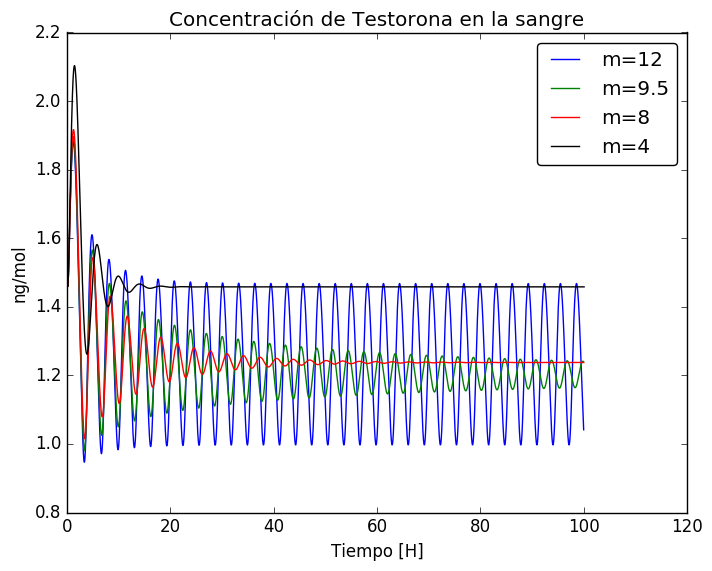
\includegraphics[width=3in]{imagenes/Graficas/testosterona1.png}
\end{center}

Haciendo lo mismo para la concentración de LHRL en la sangre se obtiene:

\begin{center}
 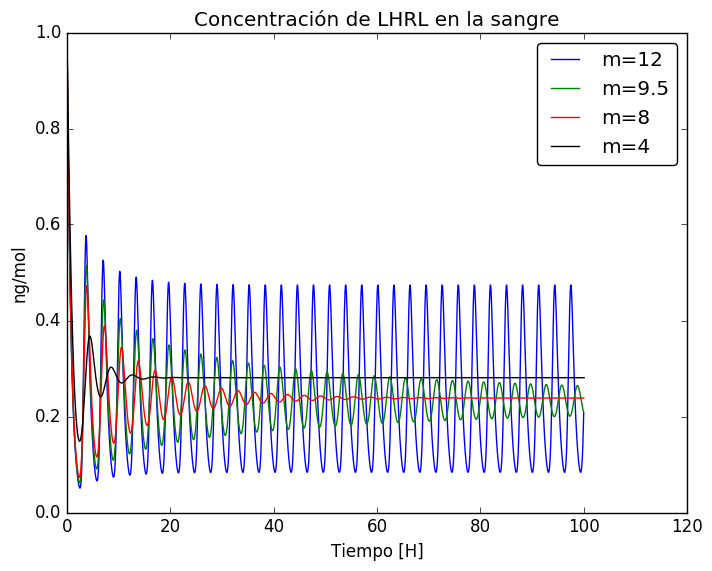
\includegraphics[width=3in]{imagenes/Graficas/LHRL1.png}
\end{center}

Y para la concentración de LH en la sangre se obtiene:

\begin{center}
 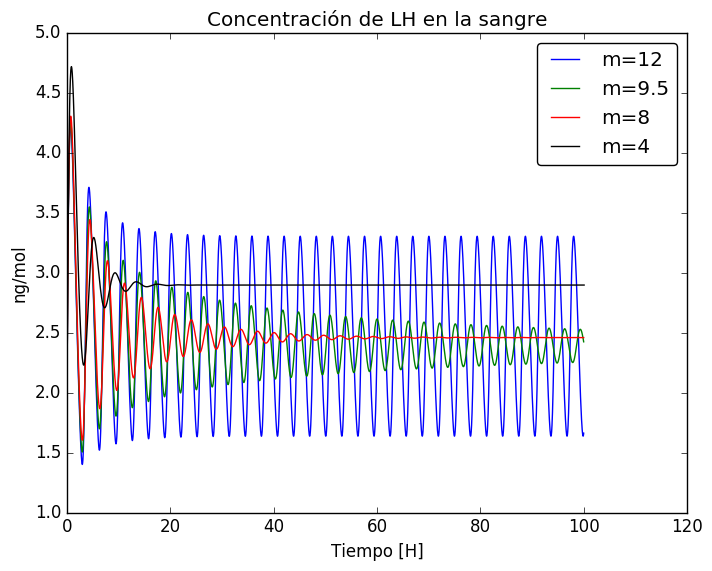
\includegraphics[width=3in]{imagenes/Graficas/LH1.png}
\end{center}

Fijando un valor para $m$ se realiza una comparación de la concentración de cada hormona en la sangre. En este caso, se toma $m=12$ y se obtiene:

\begin{center}
 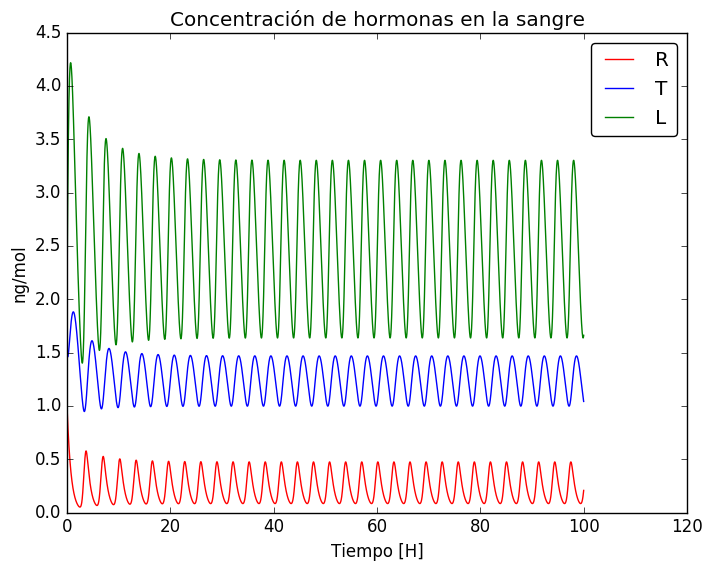
\includegraphics[width=3in]{imagenes/Graficas/hormonas1.png}
\end{center}

\begin{center}
 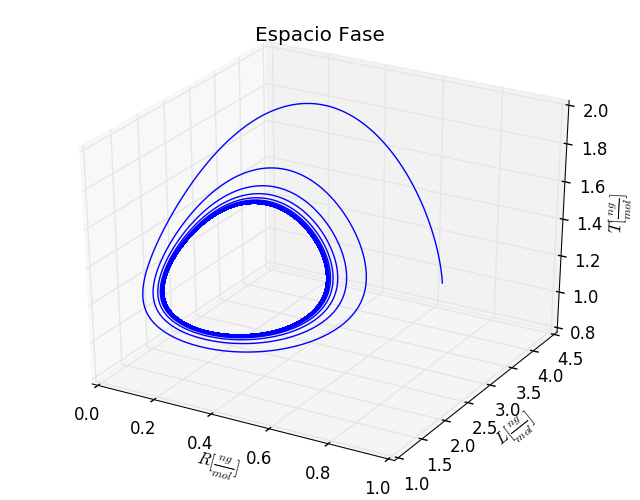
\includegraphics[width=3in]{imagenes/Graficas/hormonas2.png}
\end{center}

\section{Referencias}

[1] Murray, J. D. 1989. Mathematical Biology. Volume 19. 

[2] Smith, William R. "Hypothalamic regulation of pituitary secretion of luteinizing hormone—II feedback control of gonadotropin secretion." Bulletin of Mathematical Biology 42.1 (1980): 57-78.

\end{document}